\section{Hardware Design and Component Selection}
\label{sec:hardware}

The design of the custom actuator module is driven by a set of strict functional and physical requirements
derived from the limitations identified in the previous section.

The most critical requirement is maintaining the exact external form factor of the original servo. This
allows for a "drop-in replacement" into the existing hexapod limb structure without mechanical modification.
Consequently, all control electronics must be miniaturized to fit within the original motor chassis volume
(approx. $40 \times 20 \times 36$ mm).

The steady-state positioning error should ideally be reduced to $<\pm 0.5^{\circ}$ to enable precise
point-to-point gait control and the control interface could shift from a time-based PWM signal to a digital bus
protocol, enabling bi-directional communication (telemetry) and flexible control, while also simplifying
scalability.


\subsubsection{Position Feedback: Magnetic Encoder (AS5600)}

To eliminate the degradation issues of resistive potentiometers, the ams AS5600 \cite{as5600} magnetic rotary
position sensor was selected. This contactless sensor measures the orientation of a diametric magnet mounted
directly on the output shaft. Key advantages include:

\begin{itemize}
    \item \textbf{Contactless Operation:} Eliminates friction and mechanical wear, significantly extending
        the operational lifespan.
    \item \textbf{High Precision:} The sensor provides a 12-bit resolution over a full rotation,
        corresponding to a theoretical precision of $0.088^{\circ}$ per step ($360^{\circ}/4096$), which is
        well above the $0.5^{\circ}$ requirement.
    \item \textbf{Digital Interface:} It communicates via a robust $\text{I}^2\text{C}$ bus, reducing the
        susceptibility to electromagnetic noise inherent in analog ADC lines within the motor housing.
\end{itemize}


\subsubsection{Power Stage: H-Bridge Driver (DRV8870)}

To drive the DC motor, the DRV8870 \cite{drv8870} was chosen for its straightforward interface and integrated
protection features. Unlike the discrete transistor bridges often found in cheap servos, this integrated
H-bridge supports up to $3.6\,\text{A}$ peak current, comfortably handling the motor's stall current. The
driver allows for:

\begin{itemize}
    \item \textbf{Bi-directional Control:} Full forward/reverse driving via logic-level inputs and internal
        shoot-through protection, automatically handling the dead-time to prevent short circuits across the
        power rails during direction changes.
    \item \textbf{PWM Speed Control:} Compatible with high-frequency switching to reduce audible noise.
    \item \textbf{Integrated Protection:} Automatic current regulation (chopping) and thermal shutdown,
        protecting the electronics from stall conditions common in legged locomotion.
\end{itemize}


\subsubsection{Control Logic: Microcontroller (STM32F103C8T6)}

The "brain" of the module is the STM32F103C8T6 \cite{stm32f103c8t6}, a 32-bit ARM Cortex-M3 microcontroller.
This component was selected for its superior computational power ($72\,\text{MHz}$), necessary to execute the
real-time control algorithms, and for its comprehensive development ecosystem.

The key peripherals are the two $I^2C$ buses used for internal and external communication and interface:

\begin{itemize}
    \item \textbf{Internal Bus:} Dedicated high-speed channel for reading the AS5600 position sensor and
        interfacing with potential future on-board peripherals (e.g. EEPROM or current sensing).
    \item \textbf{External Bus:} The main interface for the actuator module. This will allows multiple
    servos to be daisy-chained on a single bus, eliminating the need for external PWM expansion boards (e.g.
    PCA9685) and simplifying the robot's wiring harness.
\end{itemize}

Additionally, the timer/PWM peripheral will accurately control the driver module.


\subsection{PCB Design and Layout}

All selected components, along with necessary passive elements (bypass capacitors, pull-up resistors, etc...),
were integrated into a custom-designed Printed Circuit Board (PCB). To respect the strict volume constraint,
the board was designed with specific dimensions to replace the original control board inside the servo case.
Additionally, an exposed 5-pin header provides access to the SWD interface (Serial Wire Debug), allowing for
firmware flashing and real-time debugging.

Detailed schematics of the board are provided in Appendix \ref{app:pcb} while the completed design can be seen
in Figures \ref{fig:pcb_layout} and \ref{fig:motor_result}. Note that provision was made for additional future
peripheral (e.g. current sensing), although outside the scope of the current experimental validation.

\begin{figure}[htbp]
    \centering
    \begin{subfigure}[b]{0.18\textwidth}
        \centering
        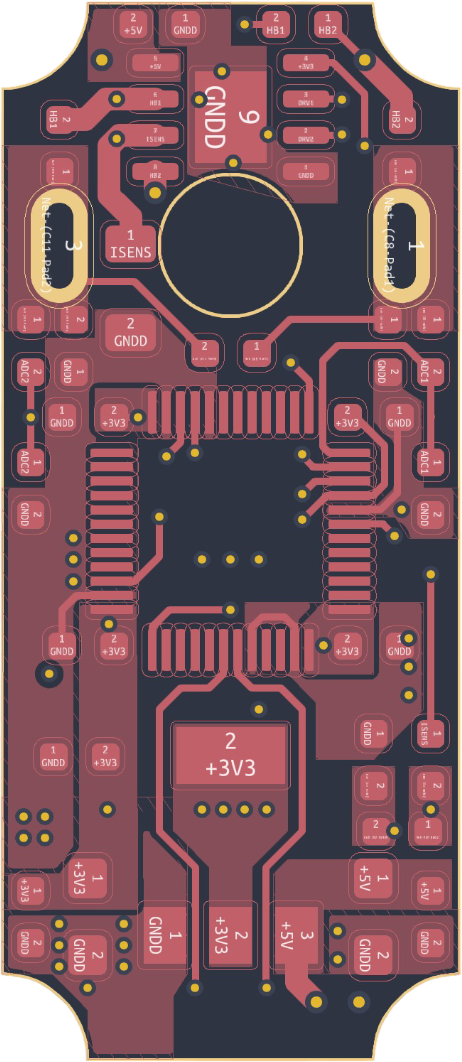
\includegraphics[width=\textwidth]{images/front_cad_pcb.png}
        \caption{CAD Front}
    \end{subfigure}
    \hfill
    \begin{subfigure}[b]{0.18\textwidth}
        \centering
        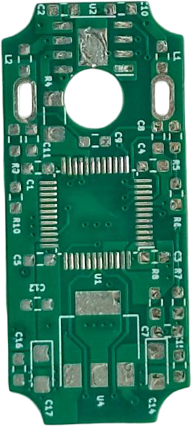
\includegraphics[width=\textwidth]{images/front_real_pcb.png}
        \caption{Real Front}
    \end{subfigure}
    \hfill
    \begin{subfigure}[b]{0.18\textwidth}
        \centering
        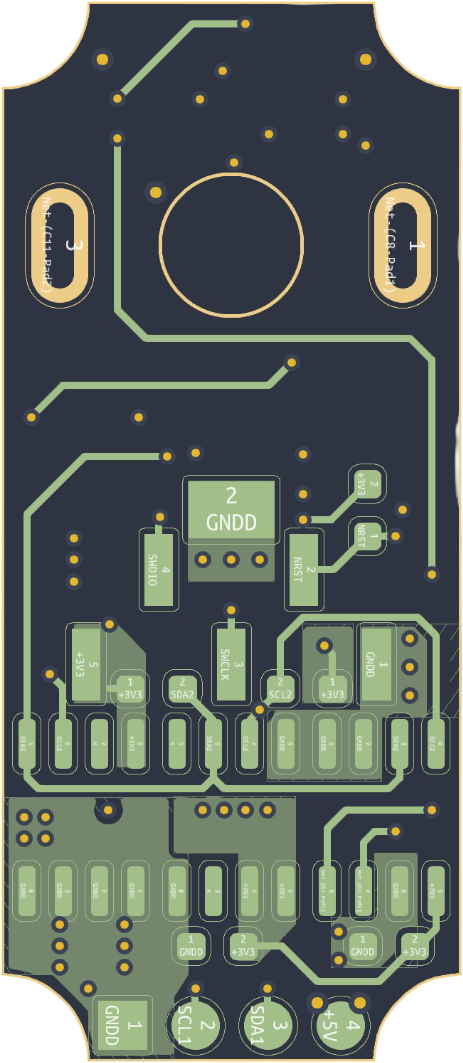
\includegraphics[width=\textwidth]{images/bottom_cad_pcb.png}
        \caption{CAD Bottom}
    \end{subfigure}
    \hfill
    \begin{subfigure}[b]{0.18\textwidth}
        \centering
        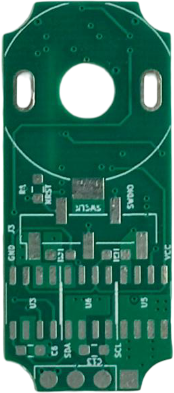
\includegraphics[width=\textwidth]{images/bottom_real_pcb.png}
        \caption{Real Bottom}
    \end{subfigure}
    \caption{Custom PCB Layout Design (CAD and Real).}
    \label{fig:pcb_layout}
\end{figure}

\begin{figure}[htbp]
    \centering
    \begin{subfigure}[b]{0.98\textwidth}
        \centering
        
\includegraphics[width=\textwidth]{images/front_motor.png}
        \caption{Front Side}
    \end{subfigure}

    \begin{subfigure}[b]{0.98\textwidth}
        \centering
        
\includegraphics[width=\textwidth]{images/bottom_motor.png}
        \caption{Bottom Side}
    \end{subfigure}
    \caption{Populated Custom PCB, i.e. Smart Actuator Internals.}
    \label{fig:motor_result}
\end{figure}